Due to the large number of interactions the mediating pseudoscalar has with the Standard Model sector, the indirect detection signals for this model are quite complex. 
In short, Dark Matter can annihilate into many final state particle pairs, and an increasing number of distinct event topologies become kinematically accessible with increasing Dark Matter mass.
Not only can the DM annihilate to various pairs of Standard Model particles, but DM may also annihilate into single SM gauge boson produced in association with an unstable Higgs sector particle, or into two Higgs sector particles. 
In turn, the Higgs sector particles will decay to pairs of SM particles, therefore the final states of DM annihilation may contain 2, 3 or 4 SM particles and the content of the dominant annihilation channel will not only depend on the Higgs sector parameters and Dark Matter mass. %Asked Linda
When fixing the coupling parameters and varying the DM mass, one can see the changes in the dominant DM annihilation channels as the different energy thresholds are crossed, as shown in this section. 

\begin{figure}[htb]
\begin{center}
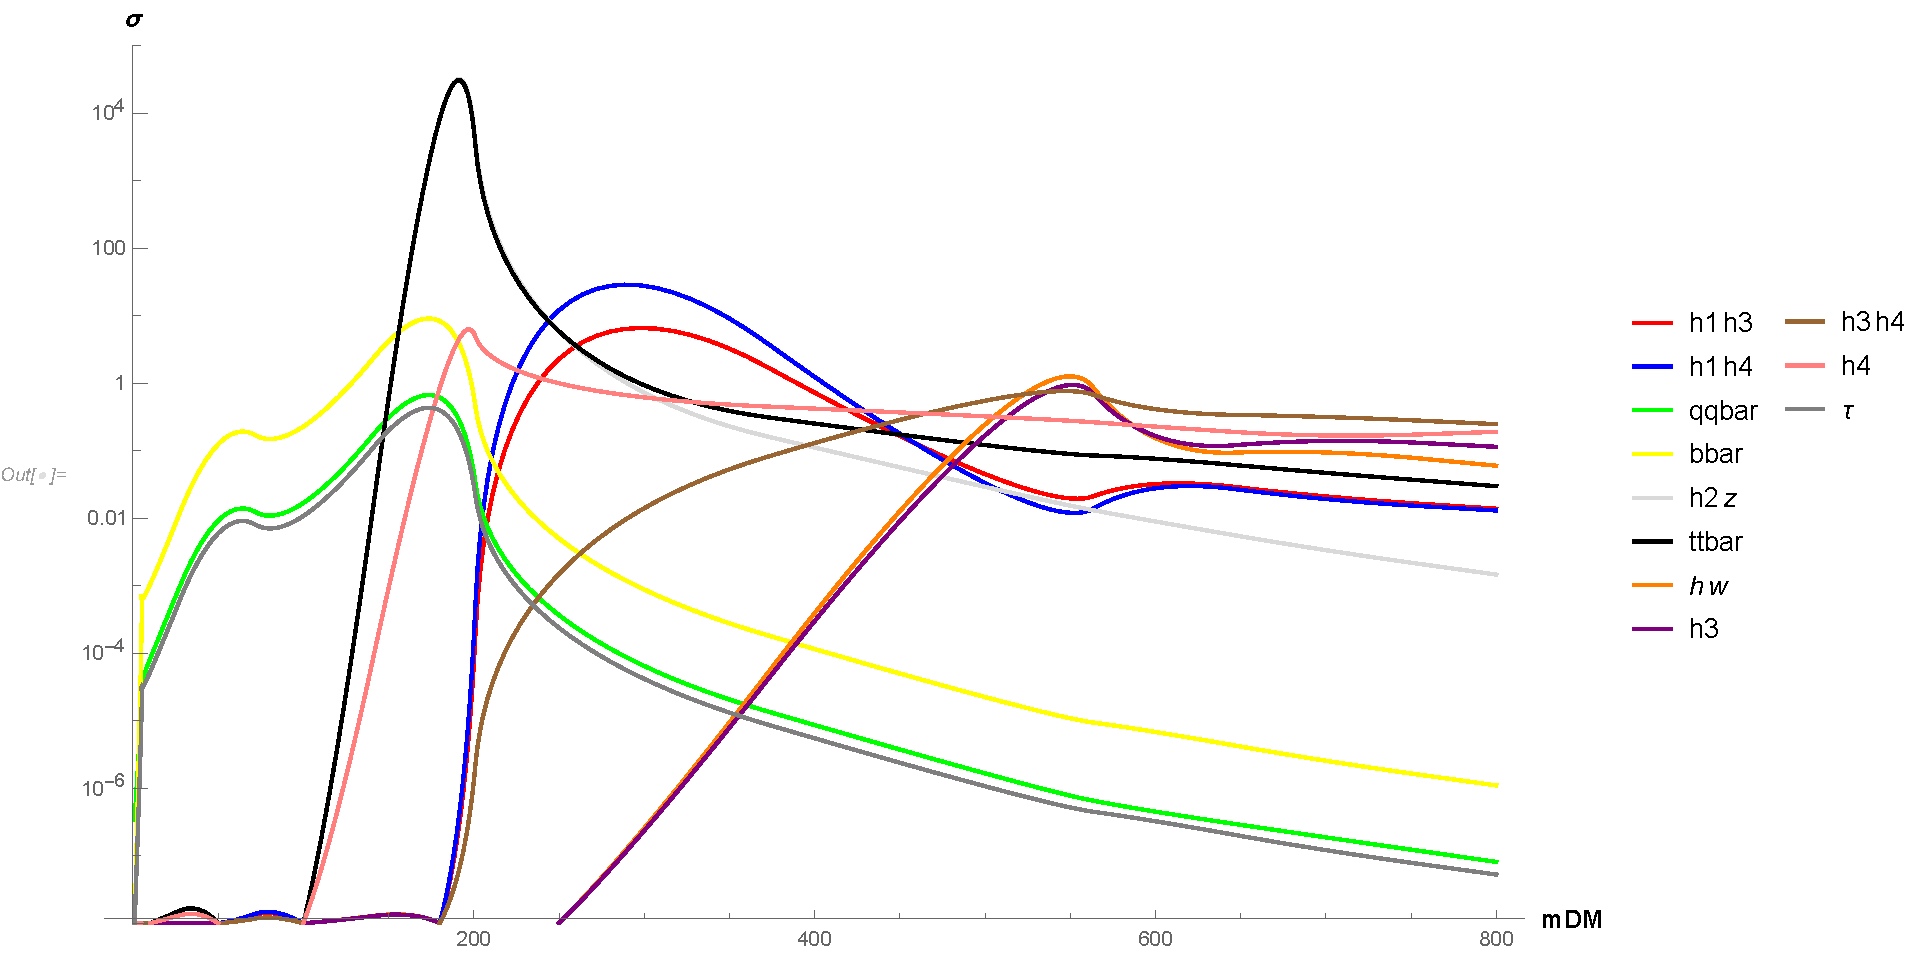
\includegraphics[width=\textwidth]{texinputs/06_comparisons/figures/indirectxsec.pdf}
\caption{A Plot of the leading Dark Matter partial annihilation cross sections, in picobarns, to various final state particle pairs, vs Dark Matter Mass (GeV). The curves include annihilation rates into fermions, pairs of Higgs sector particles, and Vector Boson-Higgs pairs.\label{fig:partialAnnihilation}}
\end{center}
\end{figure}

To illustrate the complexity of the DM annihilation channels which contribute to indirect detection, \autoref{fig:partialAnnihilation} shows the total DM annihilation rate vs Dark Matter mass for specific benchmark values of the Higgs sector parameters. 
The cross sections were calculated using the Madgraph version of the model available on the DMWG repository~\autoref{GitRepo} and the MadDM plugin\cite{Backovic:2015tpt}. 

As the DM mass in increased the dominant annihilation channel varies greatly. 
For light Dark Matter masses, under about 150 GeV, the annihilation rate is dominated by b-quark pairs, as they are the kinematically accessible particles that have the largest Yukawa coupling to the Higgs=sector mediator. 
This situation resembles the light Higgs boson decay rates, dominated by bottom quarks. 
%though the Yukawa is not particularly large, it is the only non-hopeless kinematically accessible decay. 
A new annihilation channel into a Higgs and Z boson opens when the threshold $m_{DM} \rightarrow m_h + m_Z$ is crossed. 
Next, the $m_{DM} \rightarrow m_t$, where the di-top channel opens and contributes significantly to the annihilation rate. 
The next threshold to be crossed is $2 m_{DM} \rightarrow m_a + m_h$, where the light pseudo-scalar will decay to bottom quarks. 
The event is thus likely $2 m_{DM} > 4 b$, however the momentum distribution between the two pairs of bottoms will be asymmetric. 
It is expected that the total annihilation rate into this channel is appreciable since there is a large coupling between the Higgs and the pseudoscalar which also involves mass insertion.  
This type of event topology, $DM DM \rightarrow X + SM$, where X is a decaying hidden sector particle, has not been extensively studied on its own. 
Next, the threshold $2 m_{DM} > m_V + m_H$ is crossed, where V is the mass of a heavy vector boson, and H is a heavier Higgs sector field. 
Along with all of this, modes will significantly contribute where DM annihilates to pairs of Higgs sector fields.  The most important, and lowest threshold is $ m_{DM} \rightarrow m_a$, where the annihilation channel into two pseudoscalars is open. 
There are also thresholds where DM annihilates to any pair of heavy (or one heavy and one light) Higgs sector field.

A few general notes are in order here. 
First, the effect of the new annihilation channels opening as thresholds are crossed may also be witnessed in figure 26 which charts the relic density as a function of DM mass for fixed values of the Higgs-sector parameters.  
One can see, for example, the effect of the di-top channel turning on as the overall annihilation rate is enhanced and the relic density drops. 
A similar powerful effect is observed as the threshold $2 m_{DM} \rightarrow m_a + m_h$ is crossed.  
The significant drop in relic density at this threshold demonstrates that this is an important annihilation channel which can compete or even dominate the list of partial annihilation rates. 
The annihilation rate is enhanced as the resonance thresholds $2m_{DM} = m_a, m_A$ are crossed, which will lead to stronger constraints from total photon flux measurements from indirect detection (ID) experiments.

We note that indirect detection constraints for models of the complexity of kinematics displayed here not yet been well studied. 
In much of parameter space, the annihilation cross sections are not simply dominated by a single final state channel, several distinct channels often have significant contributions.  
Since many channels will contribute to over-all photon flux and limits obtained from flux observation will require that these distinct spectra using a method similar to reference \cite{Carpenter:2016thc, Carpenter:2015xaa} to combine channels. The total photon flux expected from DM annihilations will be

\begin{equation}
\Phi_{\gamma}=\frac{1}{4\pi}\sum_{\substack{f}}\frac{\vev{\sigma_v}}{2m_{\chi}^{2}}\int_{E_{min}}^{E_{\text{max}}}\left(\frac{dN_{\gamma}}{dE_{\gamma}}\right)_{f}dE_{\gamma}J
\end{equation}

where the J-factor $(\text{GeV}^2\text{cm}^{-5})$ is the line of sight integral of the DM density $\rho$, integrated over a solid angle: $\Delta\Omega$,
$m_{\chi}$ is the Dark Matter mass, and we must sum over all accessible partial annihilation rates ${\vev{\sigma v}_{f}}$, where $f$ specifies the distinct final state. 
These predictions of total integrated flux may then be compared to observational measurements, for example of dwarf galaxies or the galactic center, which may constrain the partial annihilation rates and thus provide limits on the model parameters. 
In reference \cite{Carpenter:2016thc}, complex models with several annihilation channels were constrained using the Fermi dwarf galaxy data, where the observations of each dwarf galaxy was �stacked� in a joint-likelihood analysis. 
Such a procedure would be optimal for setting limits on this model from existing observational data. 
Below, we briefly describe the effect of various mass thresholds on the admixture of partial annihilation rates in our model.

The annihilations which involve the unstable Higgs fields will have more complicated kinematics than simple DM annihilation to 2 SM particles. Some work has been done regarding shifts in the annihilation spectrum resulting a very symmetric process where DM pairs annihilate to 2 or more identical heavy states that then decay to pairs of SM particles \cite{Elor:2015bho}.  Our model presents this as a possible annihilation process, along with others which have not yet been analysed.  These include the asymmetric process where 2 decaying Higgs sector particles of differing masses are produced and other asymmetric processes where light SM particle is produced in association with a heavier Higgs sector particle. The full parameter space of this model presents a wide area of admixtures of annihilation channels, and thus many possibilities for total integrates photon spectra.  We see that this type of 2HDM is quite complex, both in the number of annihilation channels and in kinematics as well.

%Indirect detection signals for this model are quite complex, as an increasing number of distinct event topologies become kinematically accessible as well scan from light to heavy Dark Matter masses. Not only can the DM annihilate to various pairs of standard model particles, we see from figure 24 there are two more types distinct types of event topologies with characteristic kinematics that change the number of final-state Standard Model particles in the event.  There are processes where a single SM particle is produced in association with an unstable Higgs sector particle, and processes where two Higgs sector particles are produced which decay to 4 SM particles. Here we briefly describe the important mass thresholds involved in the processes.  In many points in parameter several annihilation channels will contribute to over-all photon flux and limits obtained from flux observation will require that these distinct spectra using a method similar to reference \cite{Carpenter:2016thc}. THe total photon flux expected from DM annihilations will be
%
%
%\begin{equation}
%\Phi_{\gamma}=\frac{1}{4\pi}
%\sum_{\substack{f}}
%\frac{\vev{\sigma v}_{f}}{2m_{\chi}^{2}}\int_{E_{\text{min}}}^{E_{\text{max}}}\left(\frac{dN_{\gamma}}{dE_{\gamma}}\right)_{f}dE_{\gamma} J,
%\label{eq:gflux}
%\end{equation}
%
%where the the J-factor $(\text{GeV}^2\text{cm}^{-5})$ is the line of sight integral of the DM density $\rho$, integrated over a solid angle: $\Delta\Omega$,
%$m_{\chi}$ is the Dark Matter mass, and we must sum over all accessible partial annihilation rates $\vev{\sigma v}_{f}$, where f specifies the distinct final state. These predictions of total integrated flux may then be compared to observational measurements, for example of dwarf galaxies or the galactic center, which may constrain the partial annihilation rates and thus provide limits on the model parameters. In reference \cite{Carpenter:2016thc}, complex models with several annihilation channels was constrained using the Fermi dwarf galaxy data, where the observations of each dwarf galaxy have �stacked� in a joint-likelihood analysis.  Such a procedure would be optimal for setting limits on this model from existing observational data.  Below we briefly describe the effect of various mass thresholds on the admixture of partial annihilation rates in our model.
%
%For light Dark Matter masses, under about a 200 GeV threshold, the annihilation rate is dominated by b-quark pairs, as are the kinematically accessible particles that have the largest Yukawa coupling.  This situation is a lot like the domination of a light Higgs boson decay rate by bottom quarks, though the Yukawa is not particularly large, it is the only non-hopeless kinematically accessible decay.  A new annihilation into a Higgs and Z boson  opens up when the threshold $m_{DM} \rightarrow m_h + m_Z$ is crossed. The next threshold to be crossed is $m_{DM} \rightarrow m_t$, where the di-top channel opens which may now dominate the annihilation rate.  The next threshold to be crossed  $2 m_{DM} \rightarrow m_a + m_h$, where the light pseudo-scalar will decay to bottom quarks. The event is thus likely $2 m_{DM} > 4 b$, however the momentum distribution between the two pairs of bottoms will be asymmetric. It is expected that the total annihilation rate into this channel is appreciable since there is a large coupling between the Higgs and the pseudoscalar which also involves mass insertion.  This type of event topology, $DM DM \rightarrow X + SM$, where X is a decaying hidden sector particle, has not been well studies on its own. New Higgs sector decays will open up as the threshold $2 m_{DM} > m_V + m_H$ is crossed where V is the mass of a heavy vector boson, and H is a heavier Higgs sector field.  Along with this the production models will begin to open in which the DM annihilated to two Higgs sector fields.  The most important, and lowest threshold is $ m_{DM} \rightarrow m_a$, where the annihilation channel into two pseudoscalars will open. After this threshold, we may cross the Threshold where DM annihilated to any pair of heavy(or one heavy and one light) Higgs sector field.
%
%A few general notes are in order here. First, the effect of the new annihilation channels opening as thresholds are crossed may be witnesses in figure 26 which charts the relic density as a function of DM mass for fixed values of the Higgs-sector parameters.  WE can see, for example, the effect of the di-top channel turning on as the overall annihilation rate is enhanced and the relic density drops.  We see a similar powerful effect as the threshold $2 m_{DM} \rightarrow m_a + m_h$ is crossed.  The dramatic drop in relic density demonstrates that this is an important annihilation channel which can compete or even dominate the ;list of   partial annihilate rates.  We also note the enhancement of the annihilate rate as the resonance thresholds  $2m_{DM} = m_a, m_A$ are crossed, which will lead to stronger constraints from total photon flux measurements.  Finally we note that the complexity of kinematics displayed in this model has not yet been well studies for models of DM annihilations.  Some work has been done regarding shifts in the annihilation spectrum resulting a very symmetric process where DM pairs annihilate to 2 or more identical heavy states that then decay to pairs of SM particles \cite{Elor:2015bho}.  Our model presents this as a possible annihilation process, along with others which have not yet been analysed.  These include the asymmetric process where 2 decaying Higgs sector particles of differing masses are produced and other asymmetric processes where light SM particle is produced in association with a heavier Higgs sector particle. The full parameter space of this model presents a wide area of admixtures of annihilation channels, and thus many possibilities for total integrates photon spectra.